\documentclass[10pt]{beamer}

\usetheme{Madrid}
\usecolortheme{default}

\usepackage{amsmath}
\usepackage{amssymb}
\usepackage{booktabs}
\usepackage{graphicx}
\usepackage{hyperref}
\usepackage{pifont}
\usepackage{tikz}
\usetikzlibrary{arrows.meta,positioning}

\graphicspath{{figures/}}

\newcommand{\cmark}{\ding{51}}
\newcommand{\HYP}[1]{\textbf{Hypothesis:} #1}
\newcommand{\PLOT}[1]{\textbf{Plot:} #1}
\newcommand{\SEE}[1]{\textbf{What we see:} #1}
\newcommand{\CONFIRMED}{\begin{center}\vspace{0.15em}\textbf{\LARGE CONFIRMED}\end{center}}
\newcommand{\NOTCONFIRMED}{\begin{center}\vspace{0.15em}\textbf{\LARGE NOT CONFIRMED}\end{center}}
\newcommand{\INCONCLUSIVE}{\begin{center}\vspace{0.15em}\textbf{\LARGE INCONCLUSIVE}\end{center}}

\title{Riding Wavelets: Reproducing ``Riding Wavelets'' on Open Data}
\subtitle{Mini-project (ML for Time Series)}
\author{Janis Aiad (\texttt{janisaiad.ja@gmail.com}) \and Jordi Baroja Fernandez (\texttt{baroja.jordi@gmail.com})}
\date{MVA --- Jan 2026}

\begin{document}

\begin{frame}
  \titlepage
\end{frame}

\begin{frame}{Why this project?}
\begin{itemize}
  \item We do not work in finance: we were curious about \textbf{very noisy} data and \textbf{non-trivial spectral analysis} around extreme events.
  \item We reproduced a hedge-fund research preprint: \textbf{Aubrun et al., ``Riding Wavelets''} (jump classes via wavelets + Kernel PCA).
  \item Key motivation: markets are \textbf{non-stationary} (volatility clustering, intraday patterns) so global templates (e.g., dictionary learning) can be brittle.
  \item Goal: implement the full pipeline from the paper with \textbf{open data}, end-to-end, and test robustness across \textbf{time scales} and \textbf{markets}.
\end{itemize}
\end{frame}

\begin{frame}[fragile]{Reproducibility and engineering}
\begin{itemize}
  \item We worked 80+ hours.
  \item We wrote 2k LOC.
  \item We made 73 commits.
  \item We open-source the code.
  \item We install in one line.
\end{itemize}

\vspace{0.5em}
\begin{center}
\begin{minipage}{0.85\linewidth}
\begin{beamerboxesrounded}[shadow=true]{1-liner installation}
\begin{verbatim}
chmod +x launch.sh && ./launch.sh
\end{verbatim}
\end{beamerboxesrounded}
\end{minipage}
\end{center}
\end{frame}

\begin{frame}{Code structure (high-level)}
\centering
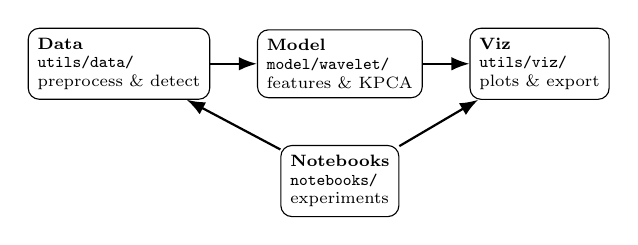
\begin{tikzpicture}[
  scale=0.85,
  transform shape,
  box/.style={draw, rounded corners, align=left, inner sep=4pt, font=\scriptsize},
  arr/.style={-Latex, thick},
  node distance=7mm
]
\node[box] (data) {\textbf{Data} \\ \texttt{utils/data/} \\ preprocess \& detect};
\node[box, right=of data] (model) {\textbf{Model} \\ \texttt{model/wavelet/} \\ features \& KPCA};
\node[box, right=of model] (viz) {\textbf{Viz} \\ \texttt{utils/viz/} \\ plots \& export};
\node[box, below=of model] (nb) {\textbf{Notebooks} \\ \texttt{notebooks/} \\ experiments};

\draw[arr] (data) -- (model);
\draw[arr] (model) -- (viz);
\draw[arr] (nb) -- (data);
\draw[arr] (nb) -- (viz);
\end{tikzpicture}

\vspace{0.25em}
\begin{itemize}
  \item We re-implement the full pipeline.
\end{itemize}
\end{frame}

\begin{frame}{Data and preprocessing}
\begin{itemize}
  \item We use 5GB Stooq OHLC equities.
  \item We cover 5-min, hourly, daily.
  \item We study Poland, Hungary.
  \item We test HK, US, UK.
  \item We normalize by local volatility.
\end{itemize}
\end{frame}

\begin{frame}{Jump detection and non-stationarity}
\begin{itemize}
  \item We standardize returns.
\end{itemize}
\[
x(t)=\frac{r(t)}{f(t)\sigma(t)}.
\]
\begin{itemize}
  \item Markets are highly non-stationary.
  \item We avoid dictionary learning.
  \item We threshold with $\theta=4$ (5-min).
  \item We assume max-stable (Gumbel).
\end{itemize}
\end{frame}

\begin{frame}{Seasonality $f(t)$ and volatility $\sigma(t)$}
\begin{itemize}
  \item Returns: $r_t=\log p_t-\log p_{t-\Delta}$.
  \item Intraday bin: $\tau(t)=$ time-of-day of $t$.
  \item Robust seasonality estimate:
\end{itemize}
\[
m(\tau)=\mathrm{median}\big\{|r_t|:\tau(t)=\tau\big\},\qquad
q=\sqrt{\frac{1}{|\mathcal{T}|}\sum_{\tau\in\mathcal{T}} m(\tau)^2},\qquad
f_t=\frac{m(\tau(t))}{q}.
\]
\begin{itemize}
  \item Deseasonalize: $r^{\mathrm{des}}_t=r_t/f_t$ (daily: $f_t\equiv 1$).
  \item Local volatility (EWMA std on $r^{\mathrm{des}}$):
\end{itemize}
\[
\mu_t=\alpha r^{\mathrm{des}}_t+(1-\alpha)\mu_{t-1},\qquad
v_t=\alpha\big(r^{\mathrm{des}}_t-\mu_t\big)^2+(1-\alpha)v_{t-1},\qquad
\sigma_t=\sqrt{v_t},\qquad
\alpha=\frac{2}{s+1}.
\]
\end{frame}

\begin{frame}{Wavelet features and interpretable directions}
\begin{itemize}
  \item We align jump signs ($t=0$).
  \item We compute complex wavelet scattering.
\end{itemize}
\[
\Phi(x)=\big(W_j\bar{x}(0),\; W_{j_2}\,|W_{j_1}x|(0)\big)_{1\le j\le J,\; 1\le j_1<j_2\le J}.
\]
\begin{itemize}
  \item We run Kernel PCA on $K(\Phi(x_i),\Phi(x_j))$.
  \item We interpret $D_1$ as reflexivity.
  \item We score mean-reversion $D_2$.
  \item We score trend $D_3$.
\end{itemize}
\[
D_2=x(-1)-x(+1),\qquad D_3=x(-1)+x(+1).
\]
\end{frame}

\begin{frame}{Gumbel diagnostic}
\small
\HYP{Jump scores are approximately max-stable (Gumbel-like) after normalization.}\\
\PLOT{Q--Q of $|x(t)|$ vs fitted Gumbel.}\\
\SEE{Overall good fit; mild 5-min tail deviation.}

\vspace{0.25em}
\centering
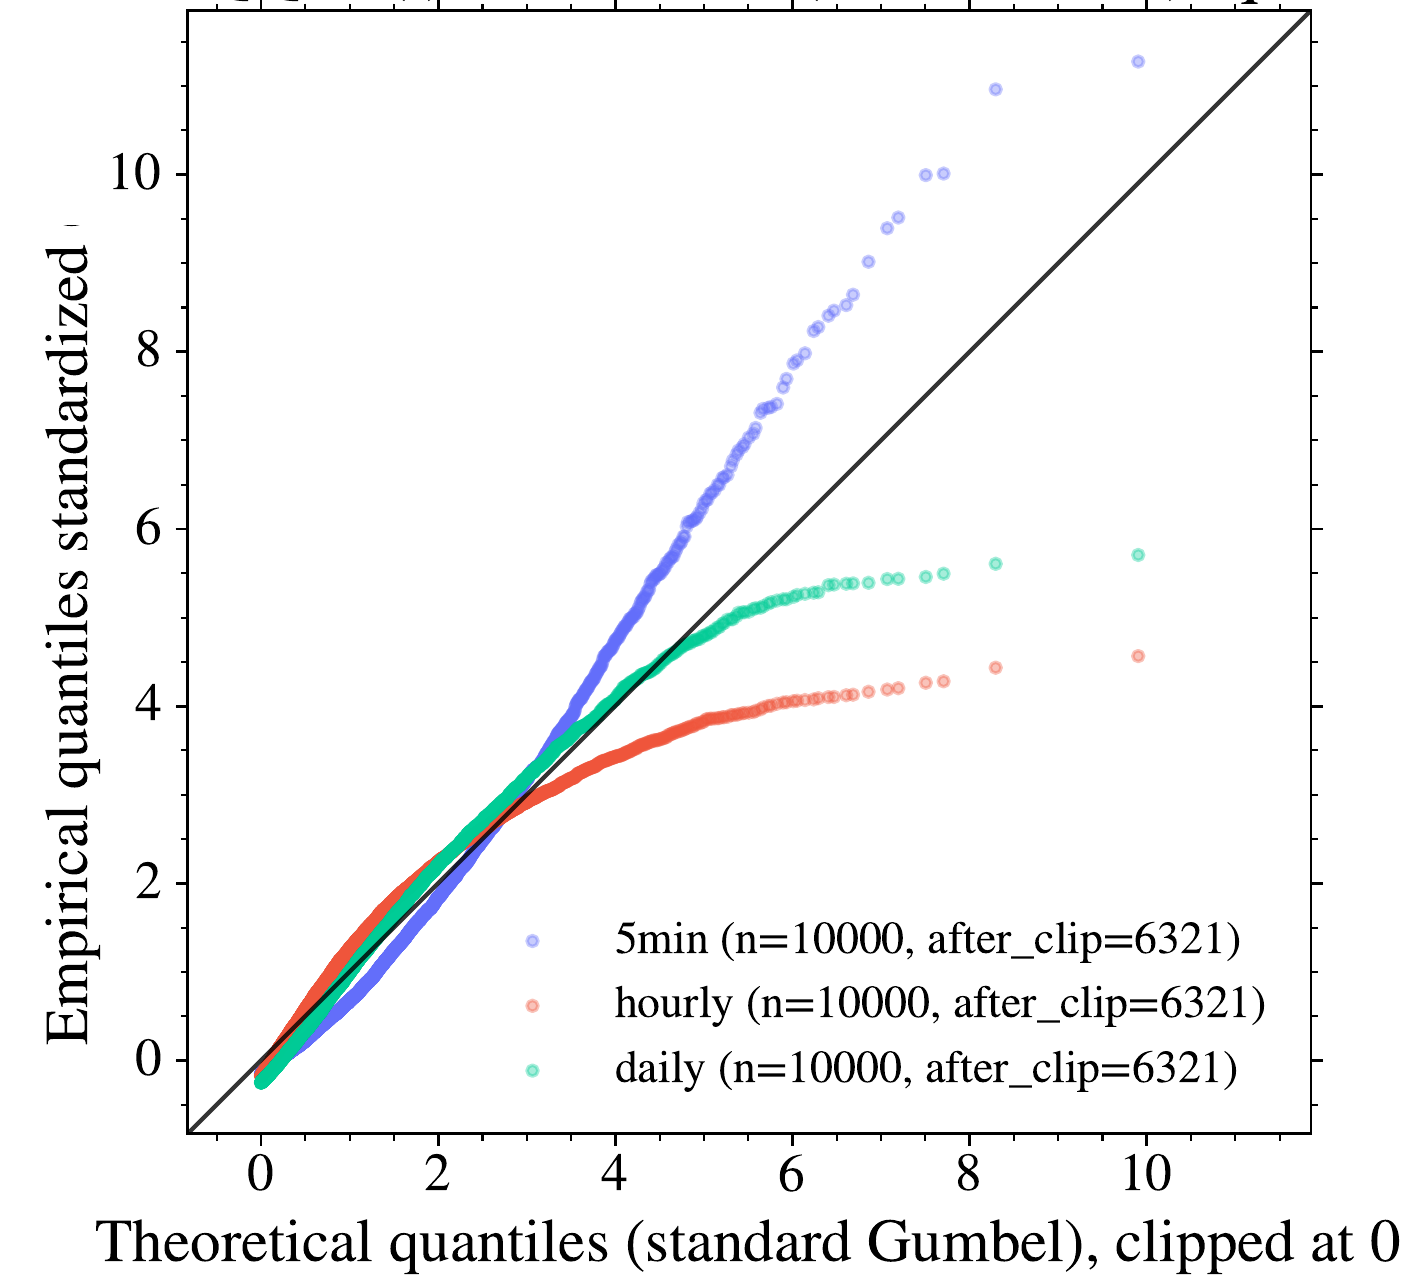
\includegraphics[width=0.98\linewidth,height=0.70\textheight,keepaspectratio]{qq_abs_score_vs_gumbel_STACKED_mpl.png}
\CONFIRMED
\end{frame}

\begin{frame}{Research question 1: robustness to the threshold (5-min)}
\small
\HYP{Average jump profiles stay stable across $\theta$.}\\
\PLOT{Overlay mean profiles across $\theta$ (5-min).}\\
\SEE{$D_1$ and $D_3$ stay stable; $D_2$ gets noisier at extremes.}

\vspace{0.25em}
\begin{columns}[T,onlytextwidth]
  \column{0.33\textwidth}
  \centering
  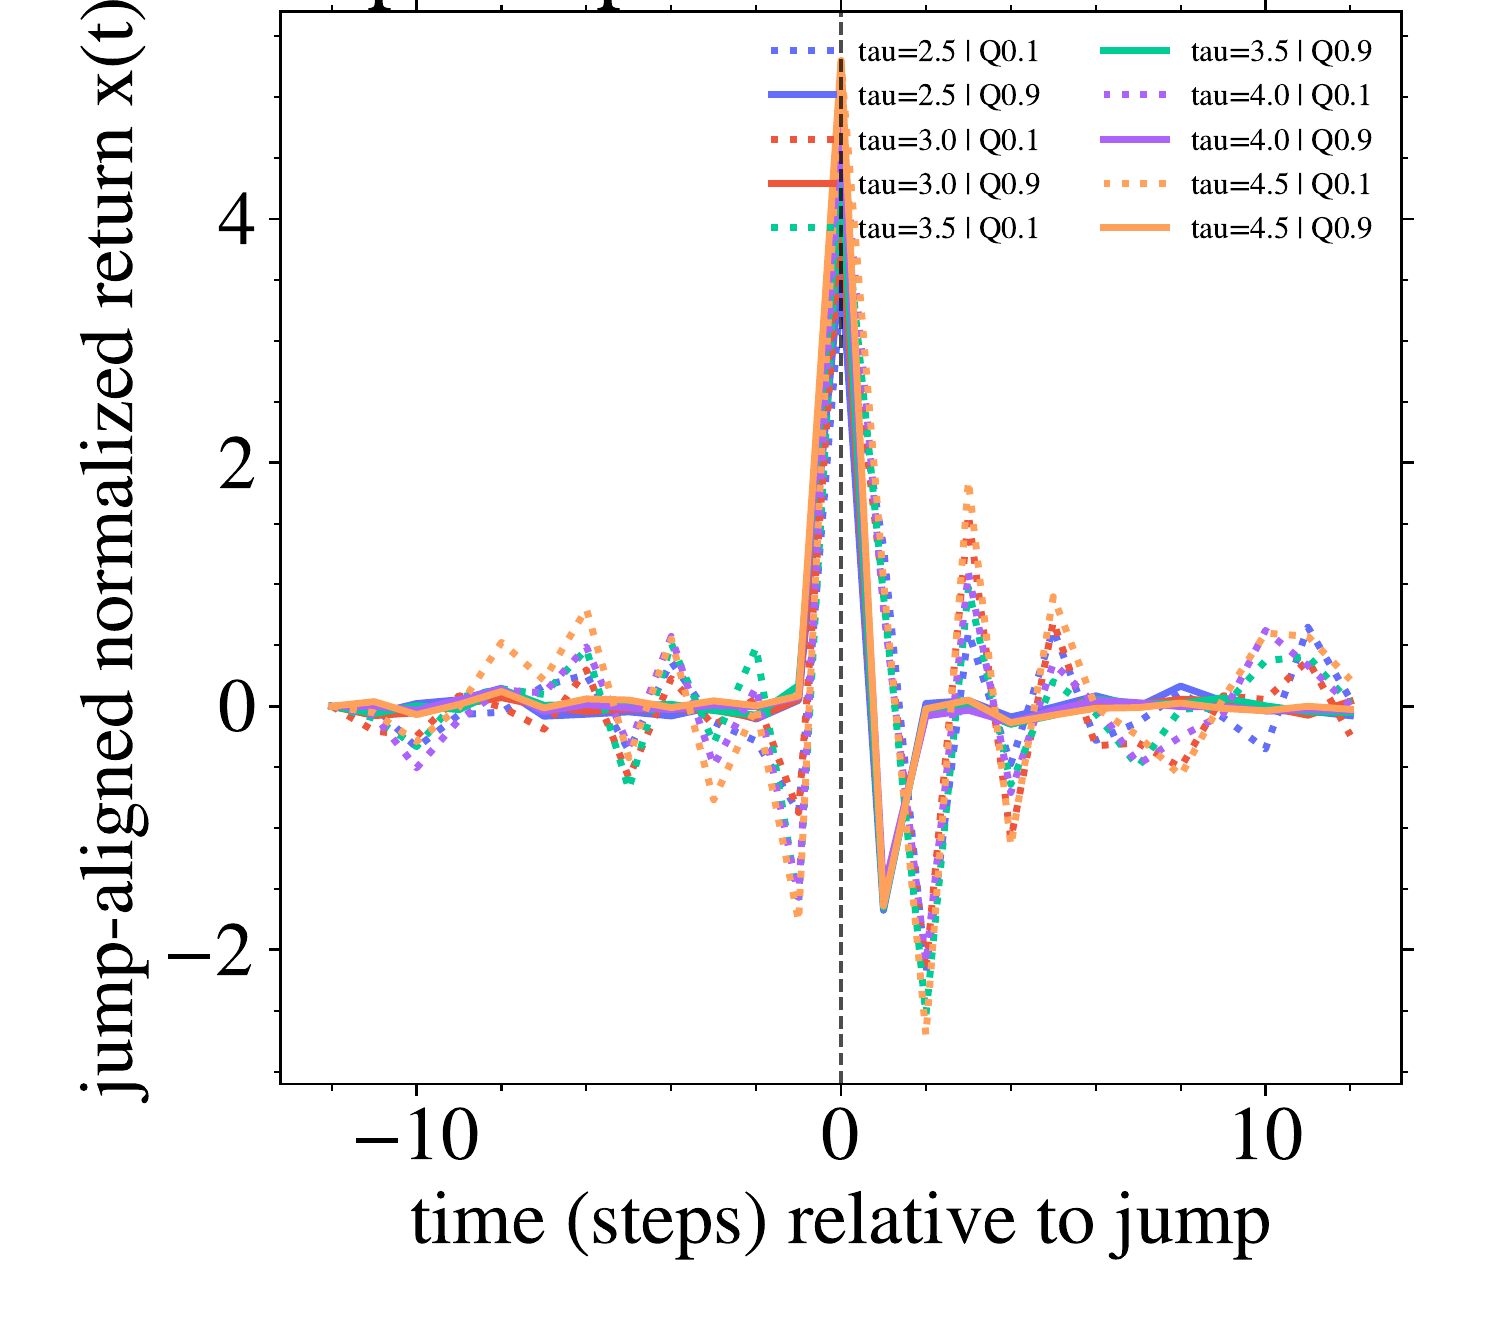
\includegraphics[width=\linewidth]{overlay_D1_thresholds_5min_mpl.png}
  {\scriptsize $D_1$ overlays}
  \column{0.33\textwidth}
  \centering
  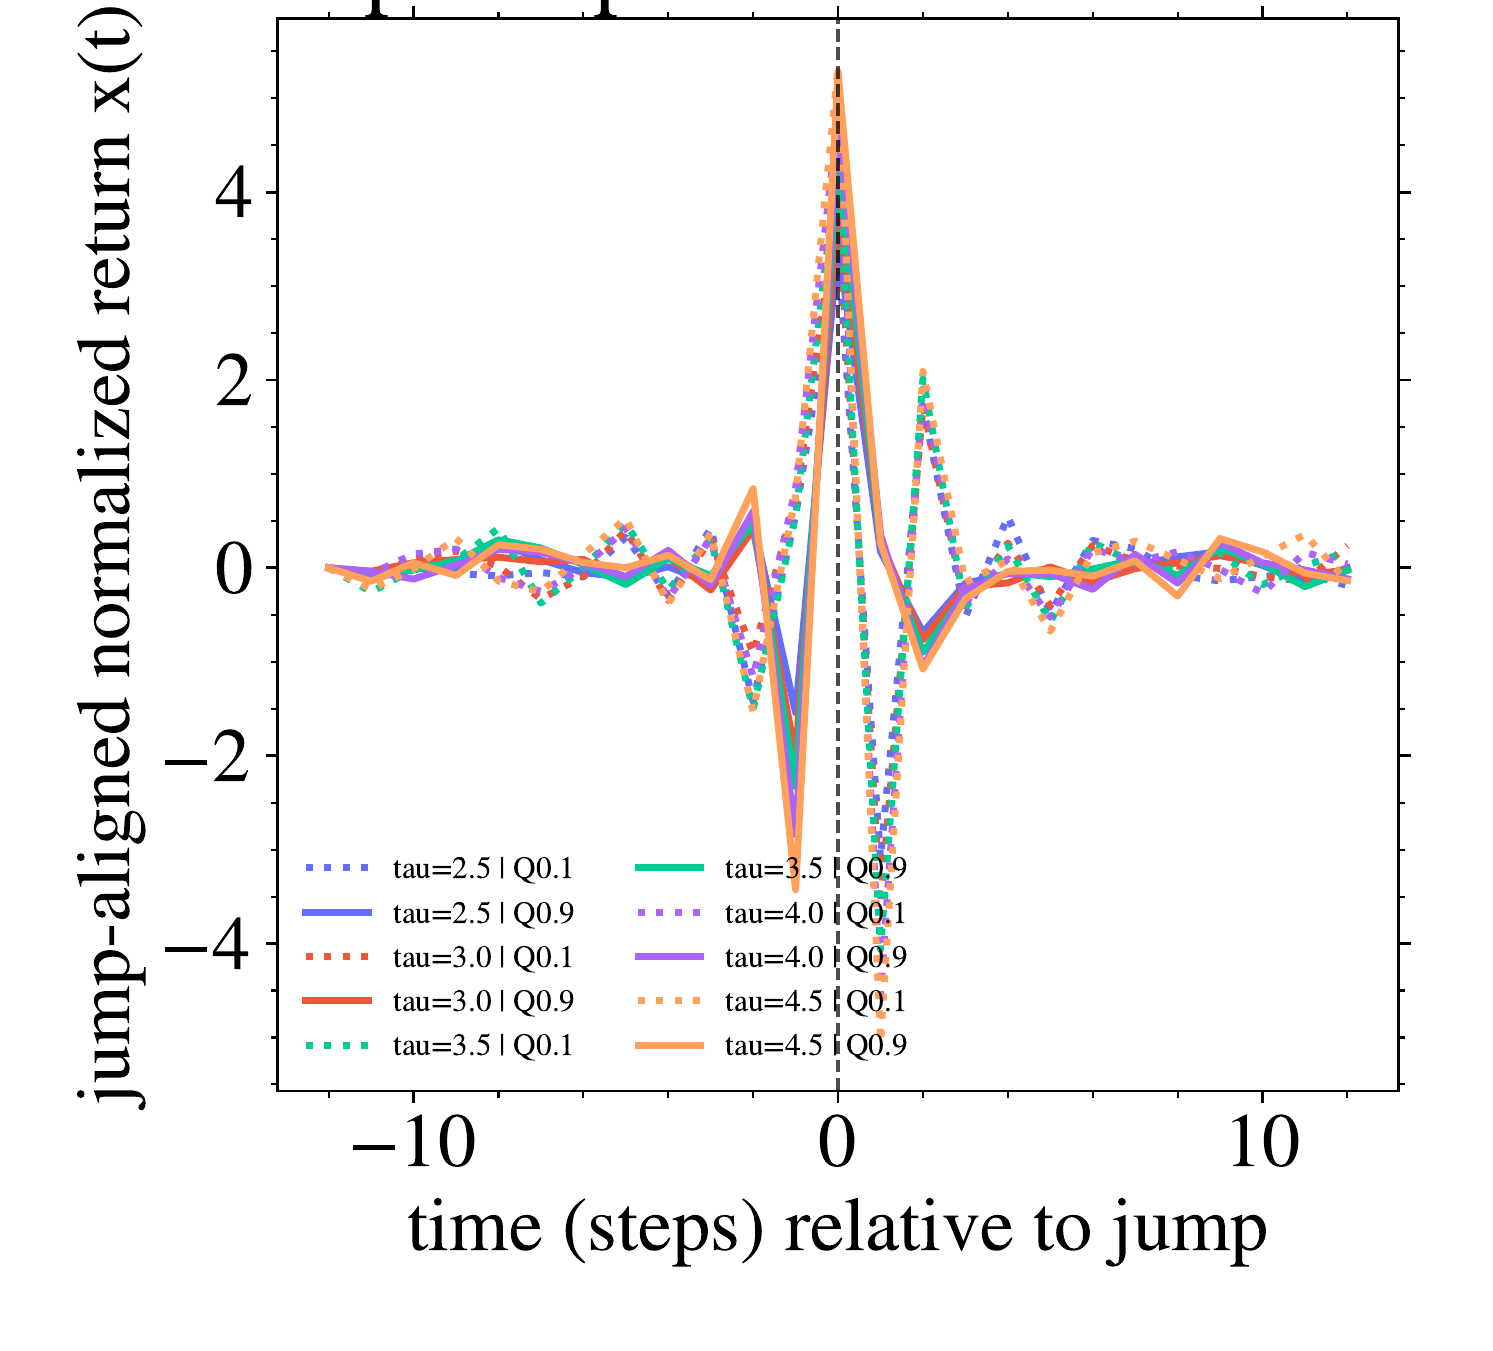
\includegraphics[width=\linewidth]{overlay_D2_thresholds_5min_mpl.png}
  {\scriptsize $D_2$ overlays}
  \column{0.33\textwidth}
  \centering
  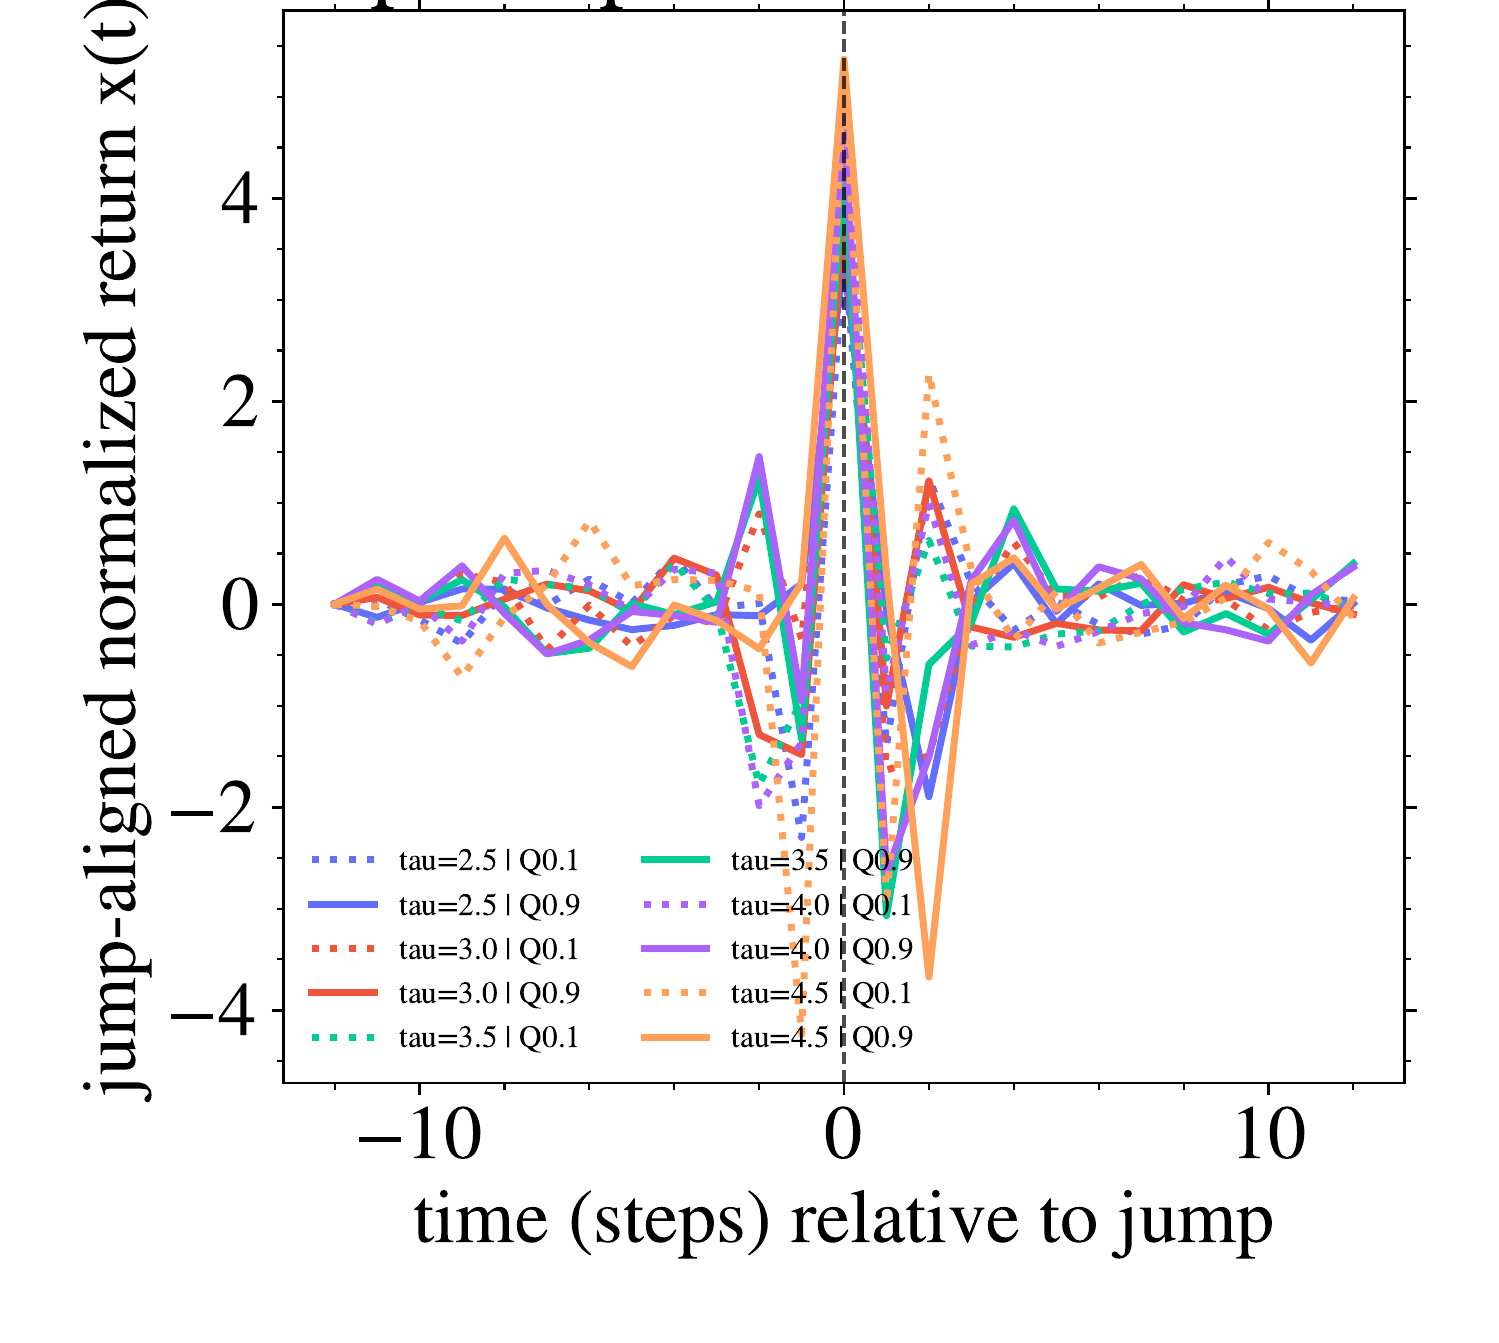
\includegraphics[width=\linewidth]{overlay_D3_thresholds_5min_mpl.png}
  {\scriptsize $D_3$ overlays}
\end{columns}
\CONFIRMED
\end{frame}

\begin{frame}{Research question 1 (cont.): daily frequency}
\small
\HYP{Same structure holds at daily scale.}\\
\PLOT{Daily overlays across $\theta$.}\\
\SEE{Profiles remain similar, with higher noise.}

\vspace{0.25em}
\begin{columns}[T,onlytextwidth]
  \column{0.33\textwidth}
  \centering
  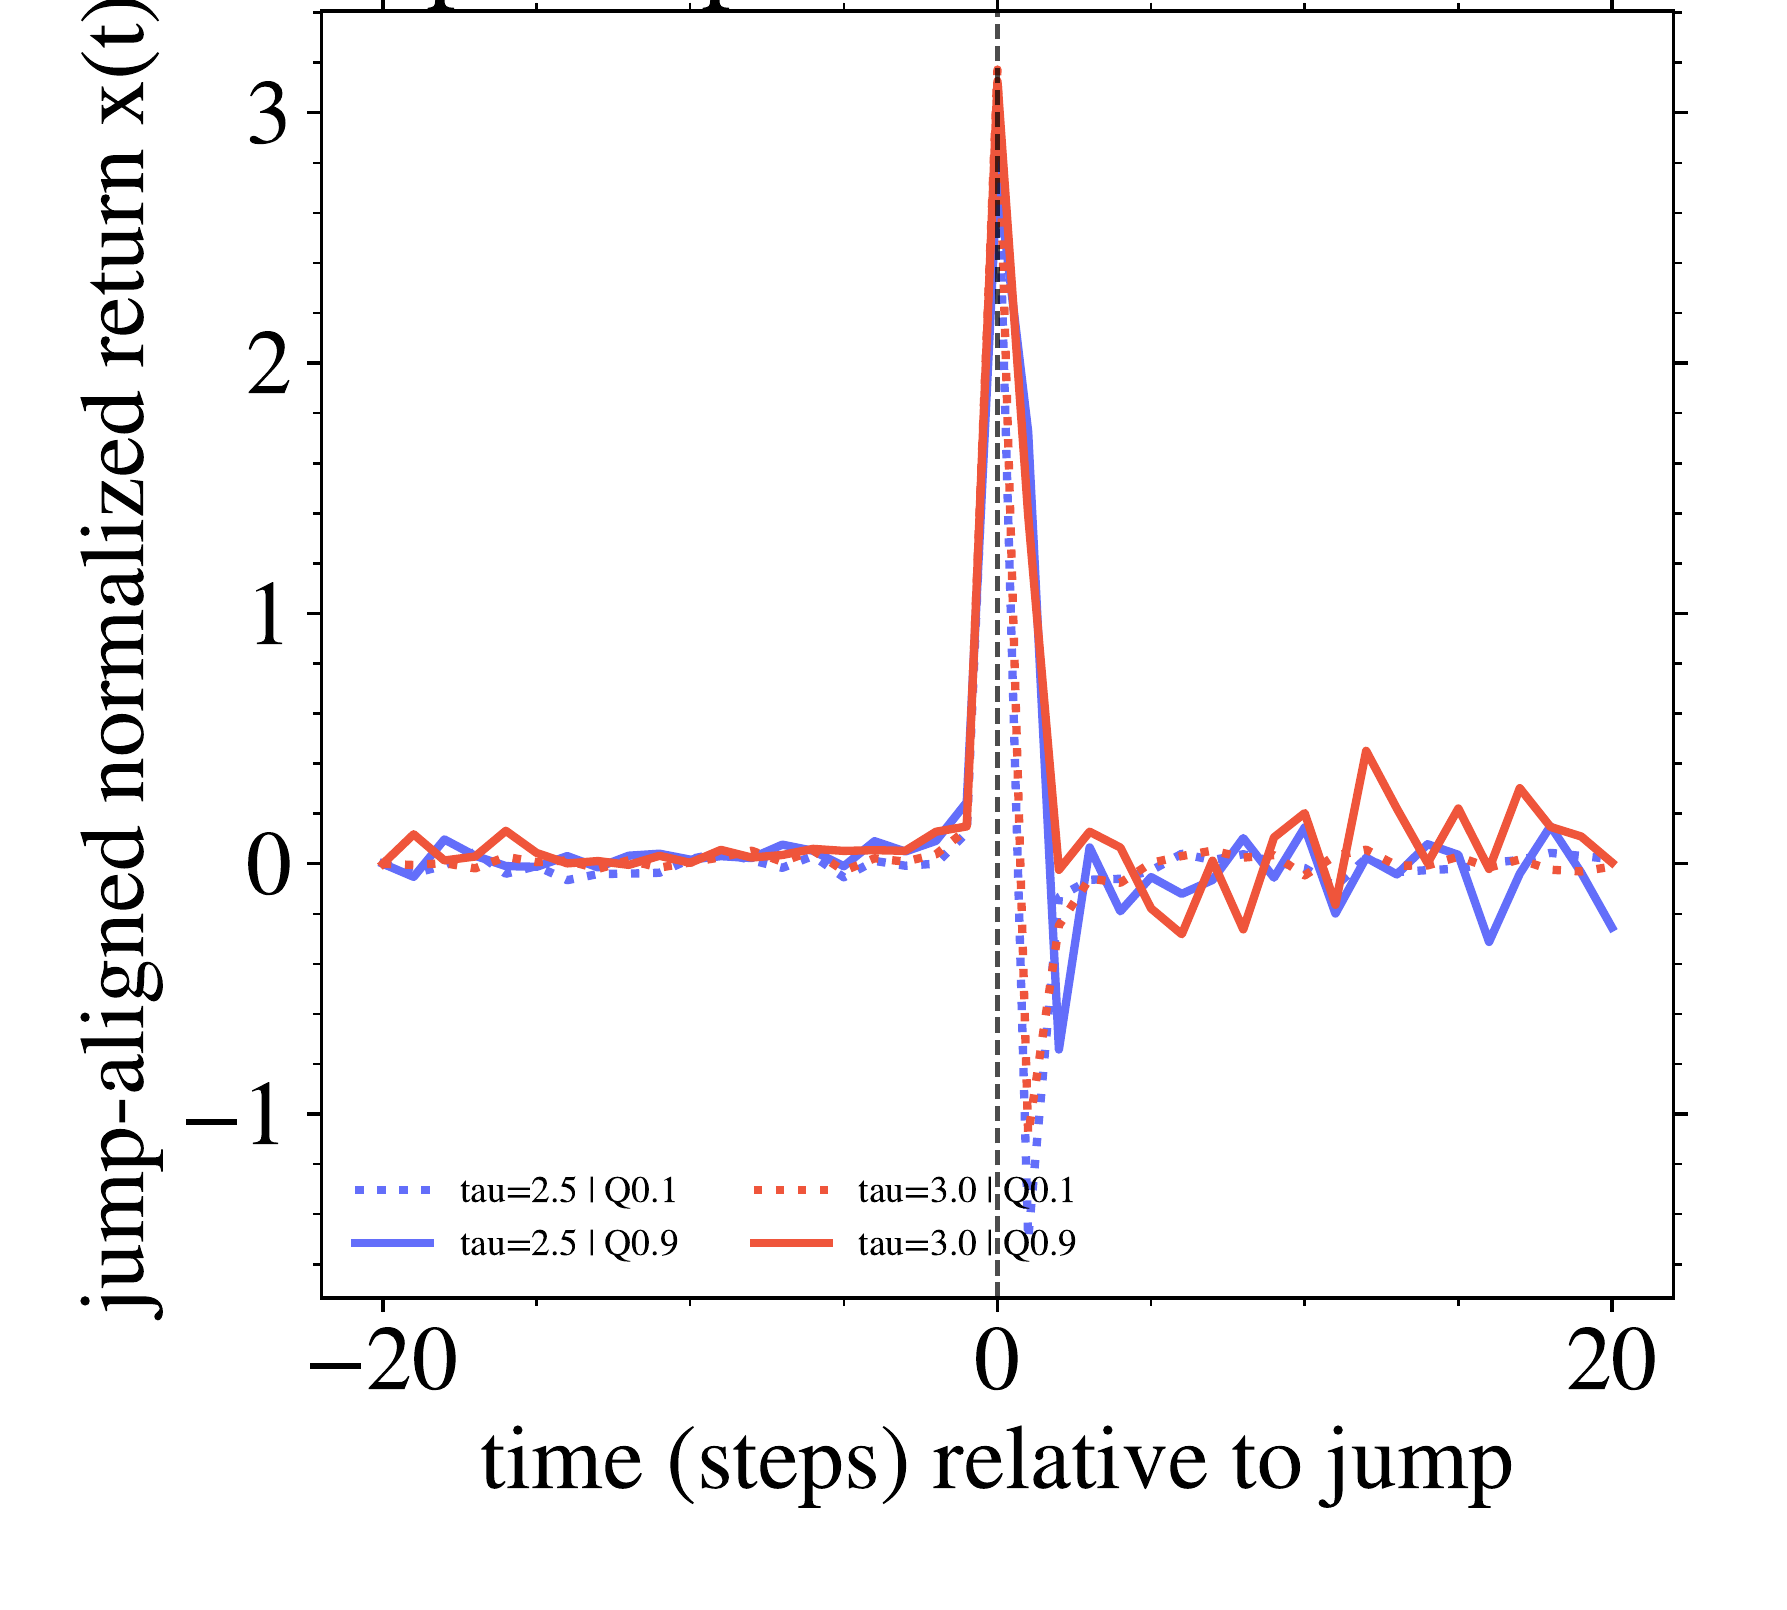
\includegraphics[width=\linewidth]{overlay_D1_thresholds_daily_mpl.png}
  {\scriptsize $D_1$ (daily)}
  \column{0.33\textwidth}
  \centering
  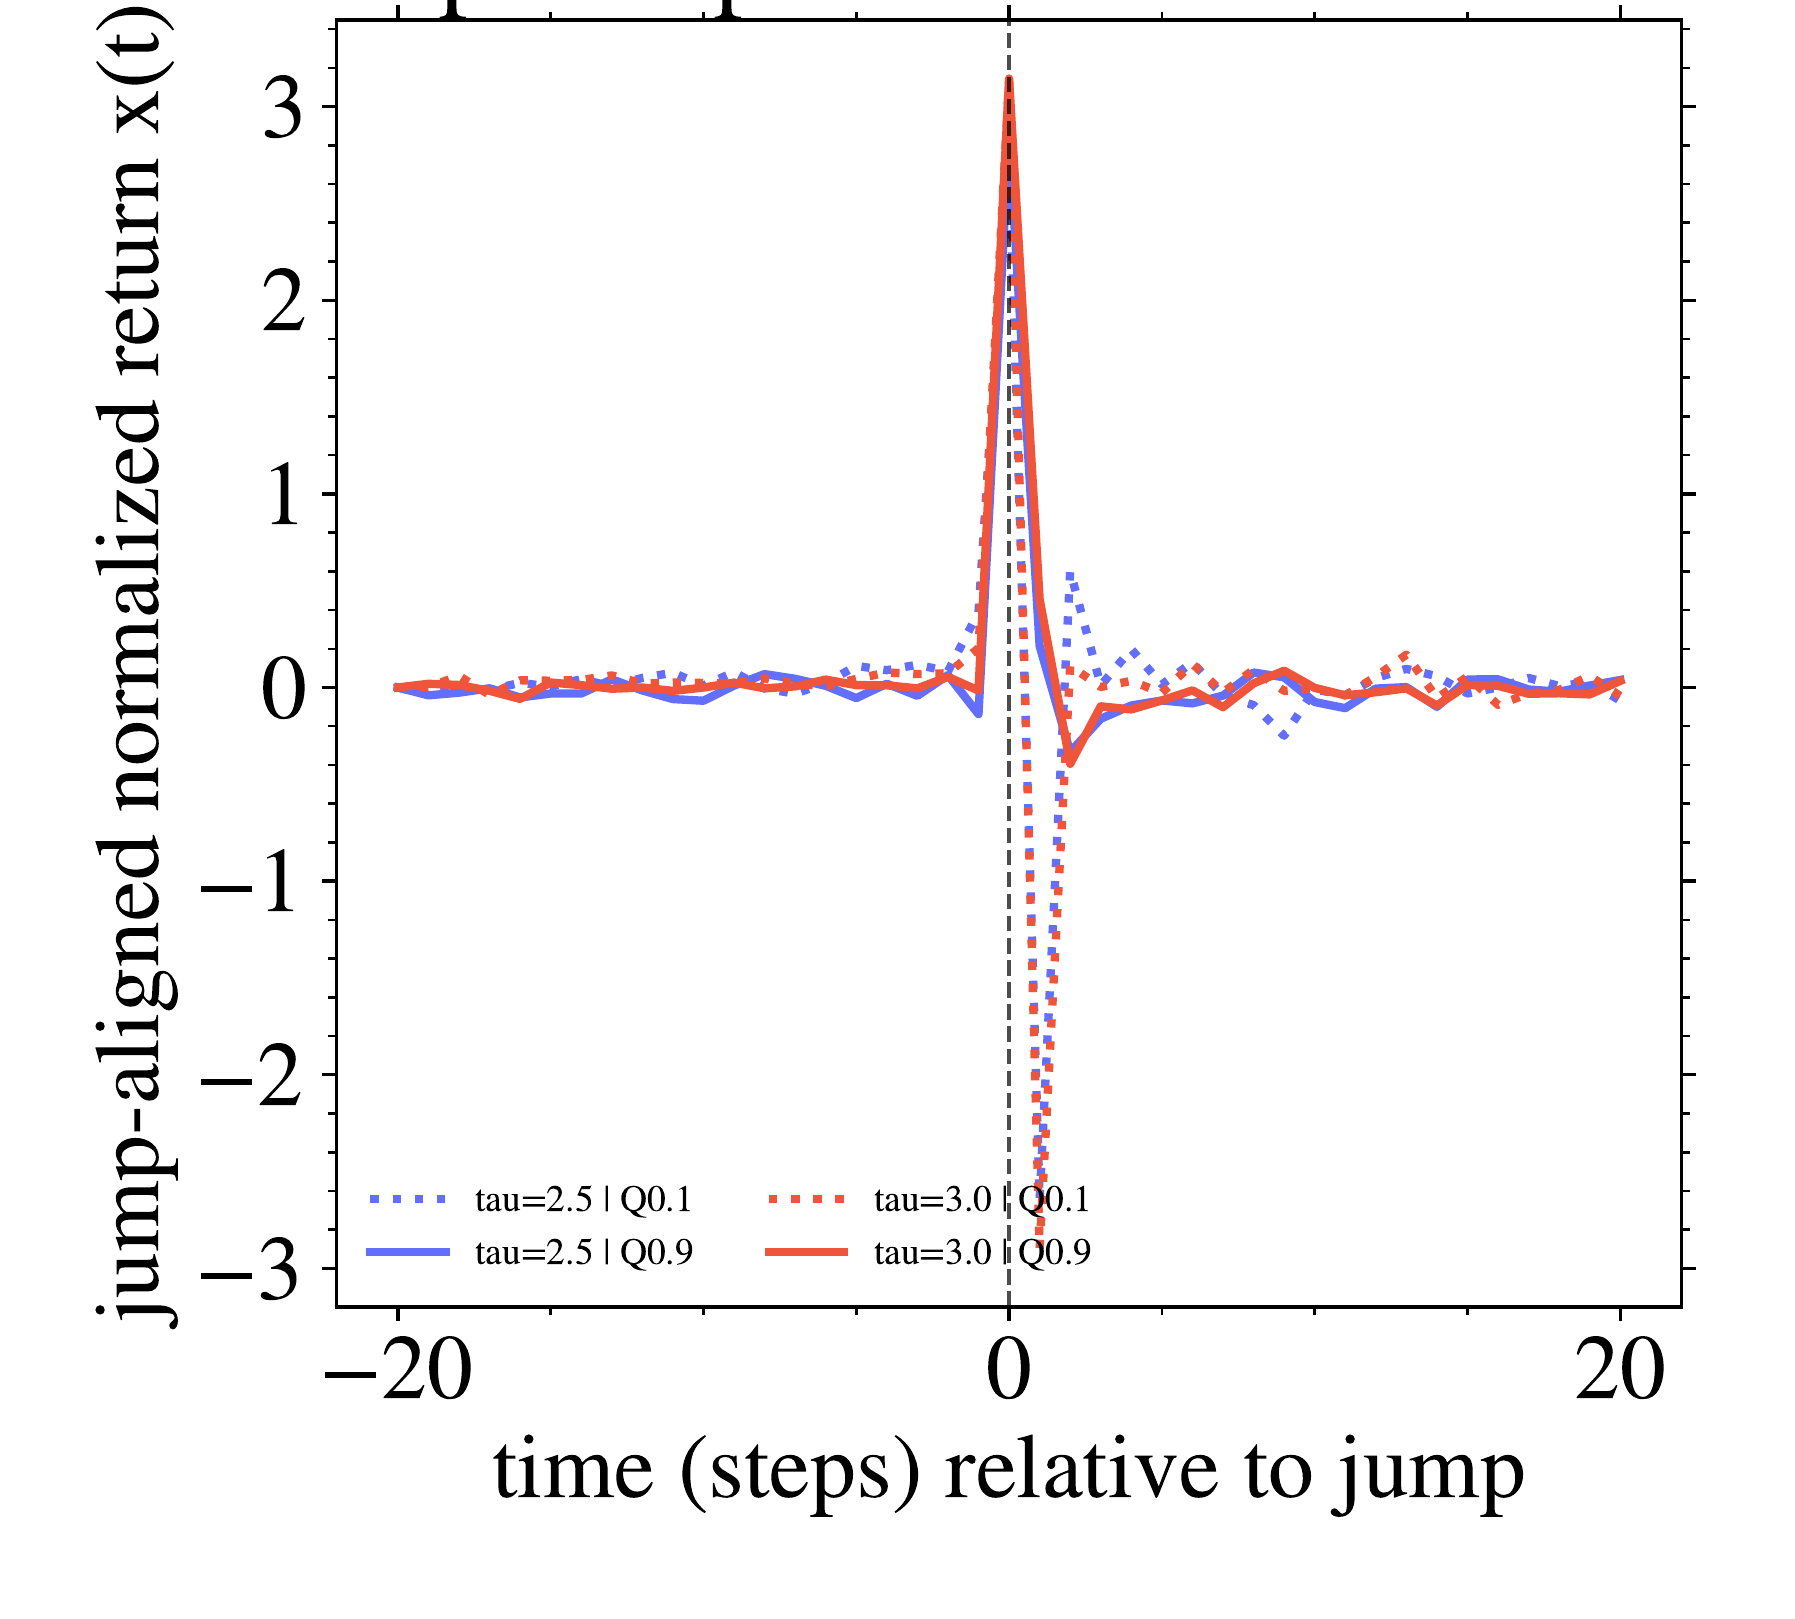
\includegraphics[width=\linewidth]{overlay_D2_thresholds_daily_mpl.png}
  {\scriptsize $D_2$ (daily)}
  \column{0.33\textwidth}
  \centering
  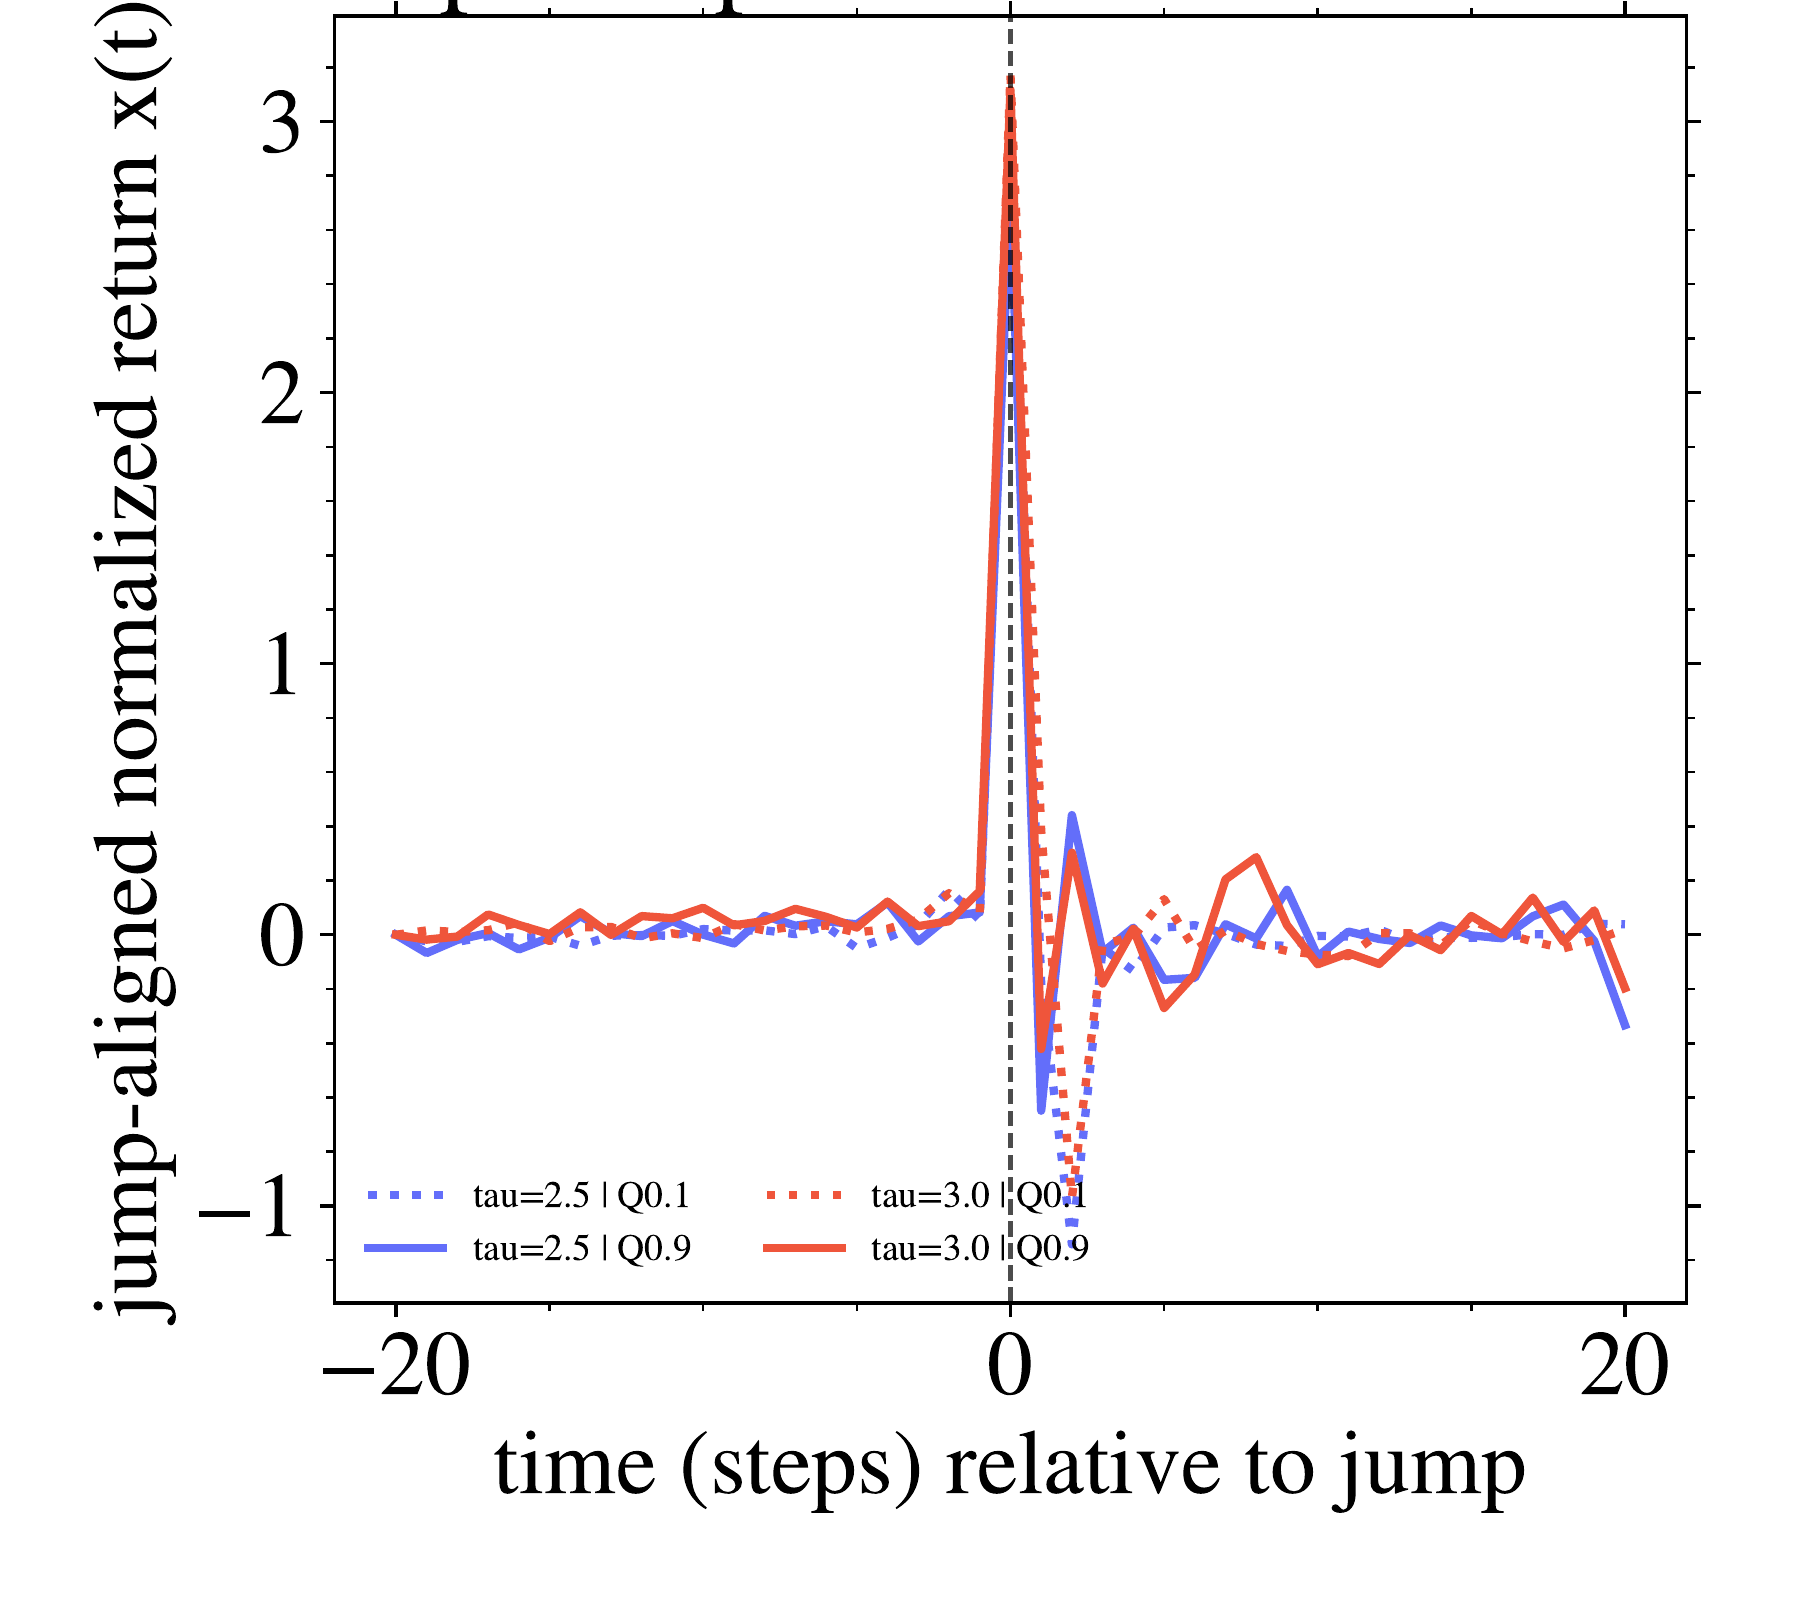
\includegraphics[width=\linewidth]{overlay_D3_thresholds_daily_mpl.png}
  {\scriptsize $D_3$ (daily)}
\end{columns}
\CONFIRMED
\end{frame}

\begin{frame}{Research question 2: do Scattering Spectra help?}
\small
\HYP{Scattering Spectra adds little at our resolution.}\\
\PLOT{With-SS vs no-SS ablation (runs).}\\
\SEE{Embeddings stay very similar; $D_1$ correlation stays high.}
\CONFIRMED
\end{frame}

\begin{frame}{Wavelet robustness: $D_1$}
\small
\HYP{$D_1$ is robust to wavelet choice.}\\
\PLOT{Different wavelet families (fbsp/cmor/cgau).}\\
\SEE{$D_1$ stays stable across wavelets.}

\vspace{0.25em}
\centering
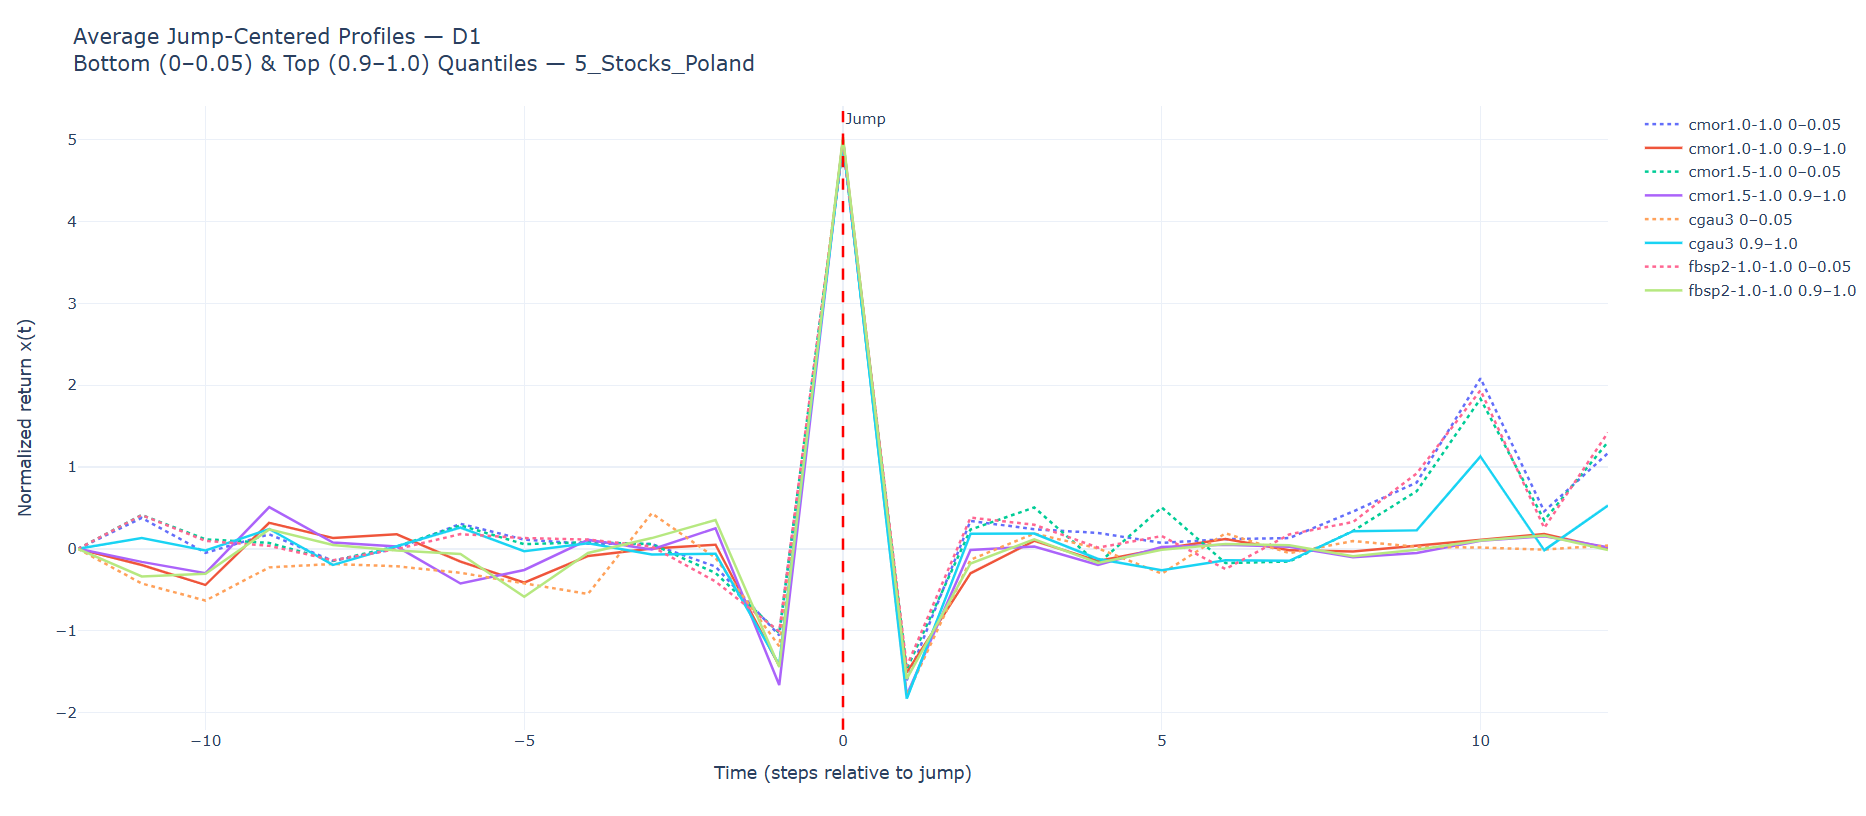
\includegraphics[width=0.98\linewidth,height=0.70\textheight,keepaspectratio]{D1_different_wavelets.png}
\CONFIRMED
\end{frame}

\begin{frame}{Asymmetry: daily vs 5-min}
\small
\HYP{Daily asymmetry correlates; 5-min does not.}\\
\PLOT{Asymmetry correlation diagnostics (daily vs 5-min).}\\
\SEE{We see strong daily correlation. We see weak 5-min correlation.}

\vspace{0.25em}
\begin{columns}[T,onlytextwidth]
  \column{0.5\textwidth}
  \centering
  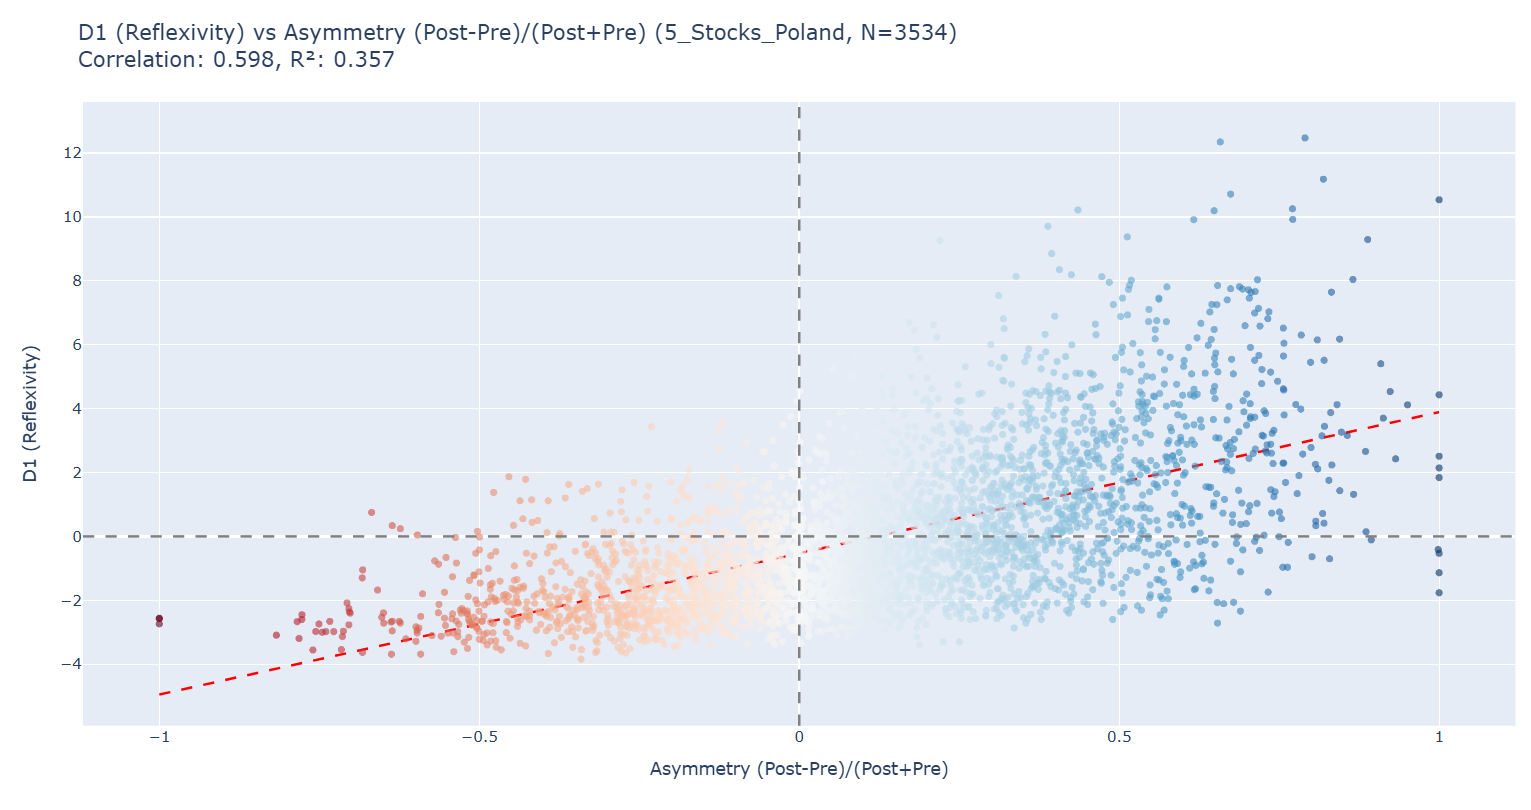
\includegraphics[width=\linewidth,height=0.68\textheight,keepaspectratio]{D1_asymmetry.png}
  {\scriptsize daily}
  \column{0.5\textwidth}
  \centering
  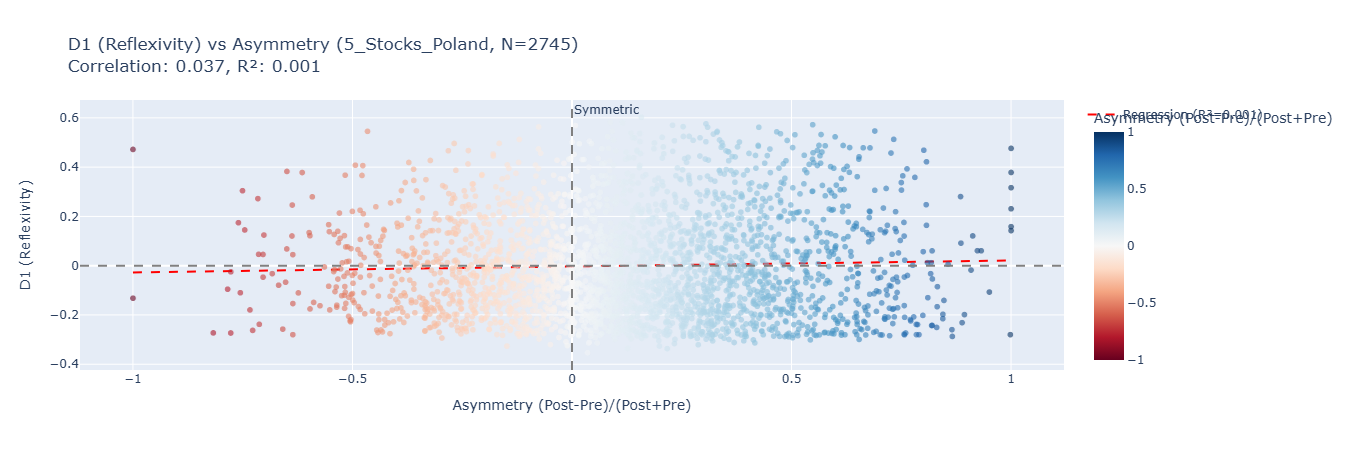
\includegraphics[width=\linewidth,height=0.68\textheight,keepaspectratio]{D1asymetry5min.png}
  {\scriptsize 5-min}
\end{columns}
\CONFIRMED
\end{frame}

\begin{frame}{Trend direction: $D_3$}
\small
\HYP{$D_3$ is a stable trend direction.}\\
\PLOT{$D_3$ profiles across wavelets / markets.}\\
\SEE{$D_3$ is unstable on PL/HU; we need more data (US placeholder).}

\vspace{0.25em}
\centering
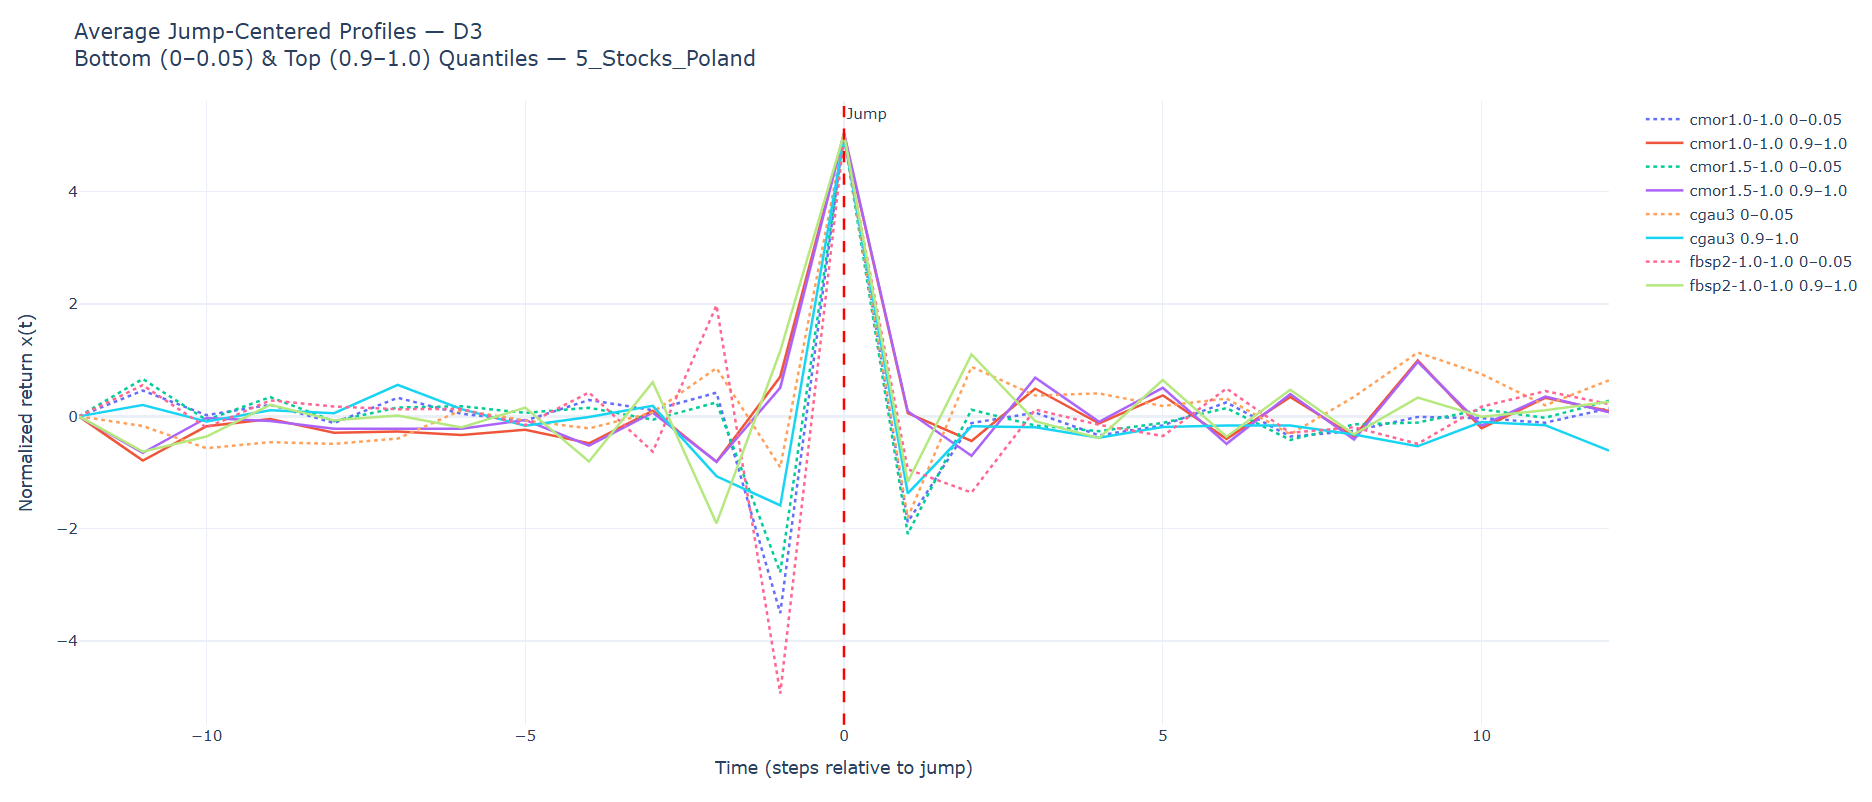
\includegraphics[width=0.98\linewidth,height=0.70\textheight,keepaspectratio]{D3_different_wavelets.png}
\INCONCLUSIVE
\end{frame}

\begin{frame}{Research question 3: robustness across markets (and co-jumps)}
\begin{itemize}
  \item We test multiple markets.
  \item We connect endo/exo signatures.
  \item We analyze co-jumps.
\end{itemize}
\end{frame}

\begin{frame}{Co-jumps: size distribution and alignment}
\small
\HYP{Co-jump sizes are heavy-tailed.}\\
\PLOT{Size histogram/CCDF and sign alignment.}\\
\SEE{Large co-jumps occur and structure emerges.}
\centering
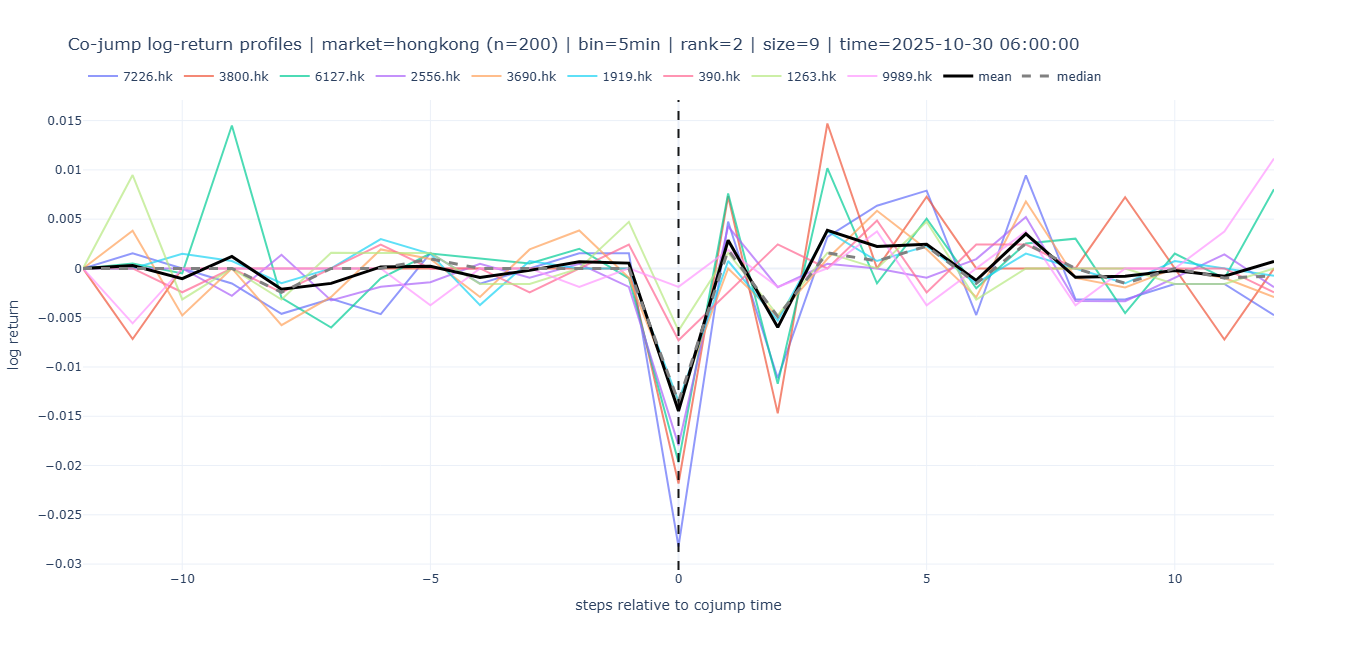
\includegraphics[width=0.98\linewidth,height=0.82\textheight,keepaspectratio]{cojump1.png}
\CONFIRMED
\end{frame}

\begin{frame}{Co-jumps: reflexivity indicator}
\small
\HYP{Large co-jumps show strong reflexivity.}\\
\PLOT{Co-jump indicator from aggregated $D_1$.}\\
\SEE{Reflexivity signal strengthens with size.}
\centering
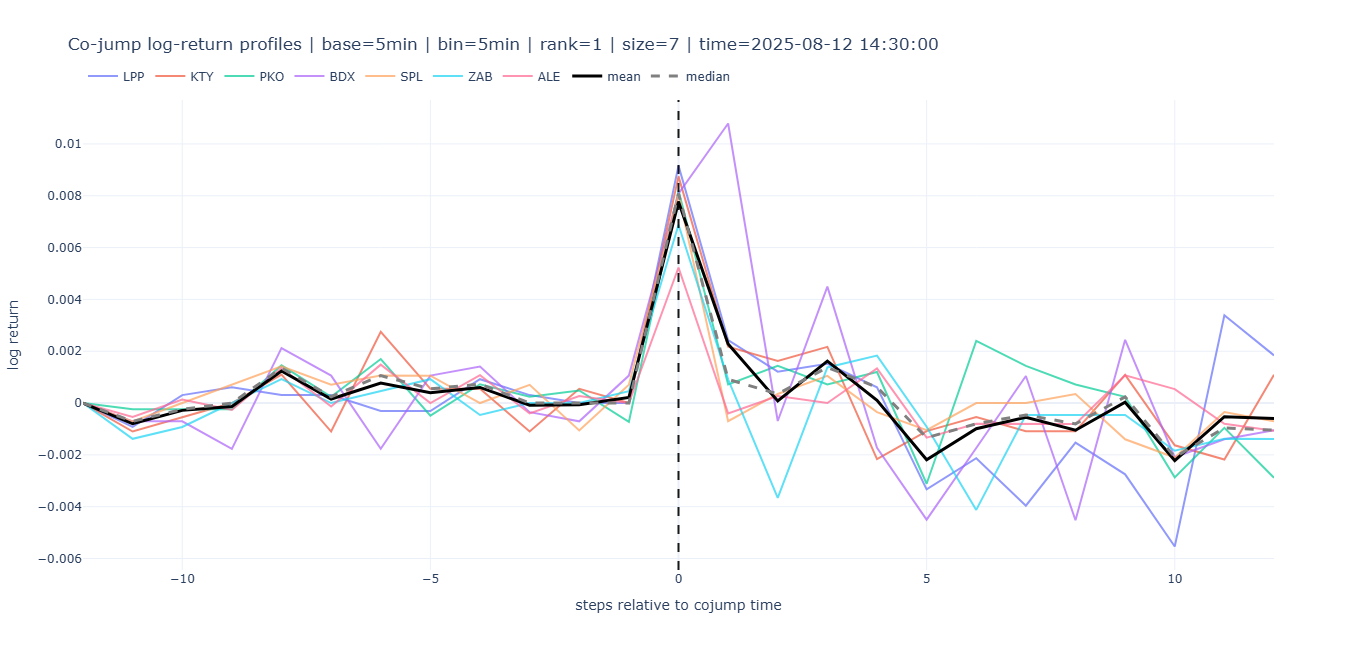
\includegraphics[width=0.98\linewidth,height=0.82\textheight,keepaspectratio]{cojump2.png}
\CONFIRMED
\end{frame}

\begin{frame}{Co-jumps: representative profiles}
\small
\HYP{Large co-jumps propagate across stocks.}\\
\PLOT{Representative constituent profiles.}\\
\SEE{Synchronized moves cluster around events.}
\centering
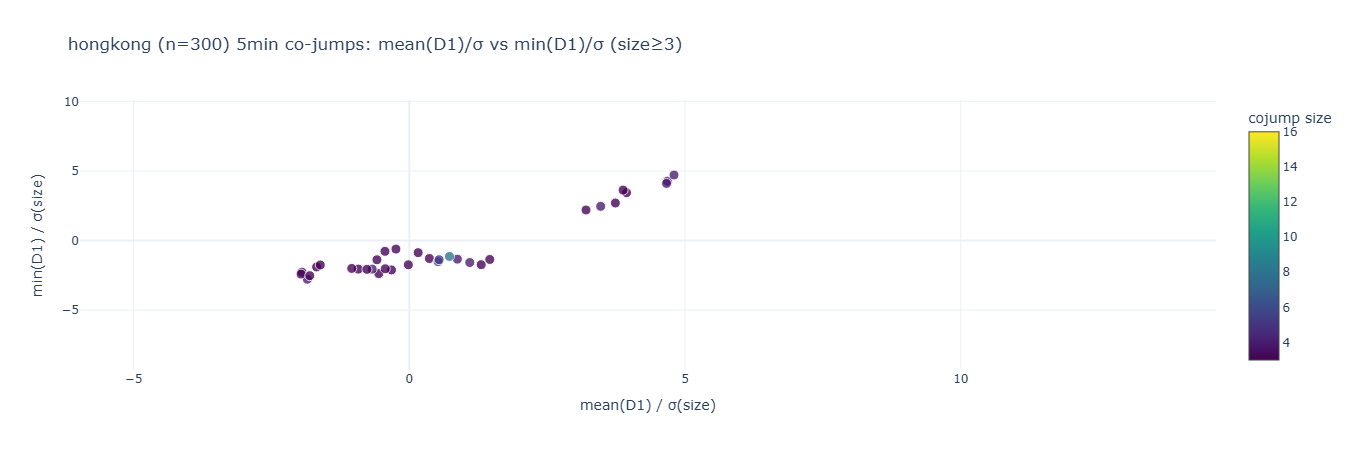
\includegraphics[width=0.98\linewidth,height=0.82\textheight,keepaspectratio]{cojump3.png}
\CONFIRMED
\end{frame}

\begin{frame}{Takeaways}
\begin{itemize}
  \item We recover jump classes.
  \item We interpret $D_1$ reflexivity.
  \item We see mean-reversion and trend.
  \item We confirm heavy tails.
  \item We confirm threshold robustness.
  \item \cmark\ We verify all the financial knowledge !! open-research is great !
\end{itemize}

\vspace{0.8em}
\centering
{\Large Questions?}
\end{frame}

\end{document}

